%*****************************************
\chapter{Peso molecolare medio}\label{ch:PM}
%*****************************************
Per ottenere il peso molecolare di una molecola bisogna vedere la tavola periodica \ref{chp:Tavolaperiodica} a pagina \pageref{chp:Tavolaperiodica}.
Ad esempio:

\begin{figure}
\subfloat[][\emph{Molecola}\label{fig:Mol}]%
{%
\setchemfig{atom sep = 2em}%
\chemfig{\vphantom{C}-[@{op,.75}]CH_2-C(-[2]CH_3)(-[6]CH_3)-[@{cl,.25}]}%
\polymerdelim[indice n]{op}{cl}}\quad
\subfloat[][\emph{Peso molecolare}\label{fig:PMmol}]%
{%
\begin{minipage}[b]{0.4\textwidth}
\begin{equation}
4*\underbrace{12}_{C} + 8*\underbrace{1}_{H} = 56\unit{\g/\mol}
\end{equation}
\end{minipage}%
}
\end{figure}

Dunque in generale si può scrivere la regola:
\begin{equation}
P.M. = P.M. * n
\label{eqn:PM}
\end{equation}

Nella realtà però, non è possibile descrivere il \ac{PM} in quanto non è detto che le catene polimeriche siano ideale e composte sempre allo stesso modo.
Dunque si stima il \ac{PMM}.

In generale la curva che descrive il \ac{PMM} per un materiale polimerico non è descritta come gaussiana ma come una curva del tipo

\begin{figure}
\centering
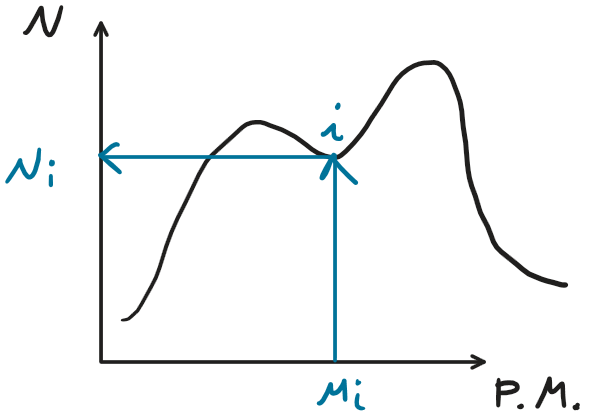
\includegraphics[width = 0.7\textwidth]{gfx/PM}
\caption{Esempio di distribuzione dei pesi molecolari in funzione del numero di moli}
\label{fig:PM}
\end{figure}

$N$ rappresenta il numero di moli con il dato peso molecolare.
In genere si hanno due massimi nella distribuzione del peso molecolare.
Le frazioni a peso molecolare più basso servono a dare al materiale delle proprietà viscose basse.
Quelle a peso molecolare alto per dare le caratteristiche meccaniche.

\section{Peso molecolare medio numerico}
Un primo parametro di caratterizzazione del polimero può essere il peso molecolare medio.
Se 
\begin{equation}
\begin{split}
W &:= \textup{Peso del campione}\\
N &:= \textup{numero totale di moli nel campione}\\
\bar{M}_n &:= \textup{Peso molecolare medio numerico}\\
\phi_i &:= \textup{Frazione molecolare}\\
\bar{M}_n &= \sum_i{\frac{W_i}{N}} = \frac{\sum_i{N_iM_i}}{N} = \sum_i{\frac{N_i}{N}M_i} = \sum_i{\phi_iM_i}
\end{split}
\end{equation}  

\section{Peso molecolare medio ponderale}
\begin{equation}
\begin{split}
\bar{M}_w &:= \textup{peso molecolare medio ponderale}\\
\psi_i &:= \textup{Frazione ponderale}\\
\bar{M}_w &= \sum_i{\frac{W_i}{W}M_i} = \frac{\sum_i{N_iM_i^2}}{W} = \sum_i{\frac{N_iM_i^2}{N_iM_i}} 
\end{split}
\end{equation}

Si può dimostrare che il peso medio ponderale è maggiore del peso medio numerico.
I due pesi medi molecolari sono uguali nel momento in cui entrambi sono uguali a un certo valore $M$.
Si può allora definire un \ac{IPD} detto anche poli-dispersità.
\begin{equation}
IDP = \frac{\bar{M}_w}{\bar{M}_n} \geq 1
\label{eqn:IDP}
\end{equation}
Dalla definizione si osserva che vale $1$ quando il polimero è mono-disperso, poli-disperso altrimenti.

Il peso molecolare medio ponderale è sensibile alle variazioni di frazioni molecolare ad alto peso molecolare.
Il peso molecolare medio numerico sensibile alle variazioni di frazioni molecolari a basso peso molecolare.

\section{Metodi di misura dei pesi molecolari}
Per la misura del peso molecolare di un campione, si scruta la dipendenza della viscosità dal peso molecolare. 
se ne estrae, tramite prove di viscosità, un peso molecolare medio. 
Si può ottenere un'ulteriore misura che permette non solo di valutare i pesi molecolari medi, consentendoci di ottenere direttamente la distribuzione dei pesi molecolari.

Non si possono ricavare con delle misure dirette i pesi molecolari, infatti le misure si realizzano sulla viscosità. 
Si parla di due tipi di viscosità: 
\begin{itemize}
\item viscosità a caldo, dove il materiale viene portato a fusione e ne misura la viscosità
\item viscosità in soluzione, dove si scioglie il materiale in un solvente con viscosità nota e si misura quella del composto misto.
\end{itemize}

\subsection{Melt Flow Index}
Il \ac{MFI} 
